\documentclass[11pt,a4paper]{article}
\usepackage{fontspec}
\setmainfont{TeX Gyre Pagella}
\newfontfamily\headfont{Inter}[UprightFont=*-ExtraBold,BoldFont=*-ExtraBold,Extension=.otf,Path=/usr/share/fonts/opentype/inter/]
\usepackage[a4paper,margin=2.3cm]{geometry}
\usepackage{graphicx,booktabs,float,caption,array,xcolor}
\usepackage[hidelinks]{hyperref}
\usepackage{titlesec}
\usepackage[round]{natbib}
\usepackage{setspace}
\setstretch{1.05}
\renewcommand{\topfraction}{0.9}
\renewcommand{\bottomfraction}{0.8}
\renewcommand{\textfraction}{0.1}
\renewcommand{\floatpagefraction}{0.75}
\setlength{\parindent}{0pt}
\setlength{\parskip}{0.55em}
\titleformat{\section}{\headfont\Large}{\thesection}{0.8em}{}
\titleformat{\subsection}{\headfont\large}{\thesubsection}{0.8em}{}
\captionsetup{font=small,labelfont=bf}
\urlstyle{same}
\hypersetup{pdftitle={Life on the Moving Map: 540 Million Years of Animal Fossils on the Drifting Continents},pdfauthor={Tristan Hotham}}

\begin{document}
\begin{center}
{\Large\bfseries Life on the Moving Map\par}
\vspace{0.4em}
{\large 540 million years of animal fossils on the drifting continents,\\from the Paleobiology Database and the PALEOMAP plate model\par}
\vspace{1.2em}
{\large Tristan Hotham\par}
\vspace{0.3em}
{\small Independent researcher\\
ORCID: 0000-0003-4931-9349\\
DOI: \href{https://doi.org/10.5281/zenodo.23856870}{https://doi.org/10.5281/zenodo.23856870}\par}
\vspace{0.8em}
2026
\end{center}

\begin{quote}
\small
\begin{center}\textbf{Abstract}\end{center}
Every fossil has two locations: where it is found today and where the animal lived, which plate tectonics has since moved. I place 409,895 fossil occurrences of 24 animal groups, from trilobites to hominids, from the Paleobiology Database at their ancient positions, computed with the PALEOMAP plate model, and draw them on PALEOMAP continental outlines for 66 ages from 540 million years ago to today. I describe the assembly and break-up of Pangaea with a simple index, the share of all land in the largest connected land mass, which exceeds 85\% from 270 to 180 million years ago and peaks at 90.2\% at 180 million years ago (today 54.4\%). Counting distinct genera in 5 million year bins, trilobites make up 57\% of Paleozoic genera in these groups, insects 42\% of Mesozoic and mammals 39\% of Cenozoic genera. Dinosaur genera from the Late Triassic and Early Jurassic, when Pangaea was whole, are found on more than one present-day continent more than twice as often (11.3\%) as Cretaceous genera (5.1\%). A simple last-appearance measure picks out the end-Permian (74.4\% of genera last seen) and end-Cretaceous extinctions but not the end-Triassic. Throughout, the record is strongly shaped by where palaeontologists work: 66\% of occurrences come from North America and Europe, which hold 32\% of the land. An interactive map lets readers move through time, switch any fossil between its ancient and present-day position, and search for genera.

\textbf{Keywords:} palaeogeography; fossil record; Paleobiology Database; PALEOMAP; Pangaea; dinosaurs; mass extinctions; sampling bias; data visualisation
\end{quote}

\section{Introduction}
Continents move a few centimetres a year. Over the 540 million years since animals with hard parts became common, that is enough to carry a piece of crust from the southern tropics to the Arctic, to gather nearly all land into one supercontinent, Pangaea, and to break it apart again. Fossils travel with the rocks that hold them. A trilobite found in Wales, a coal-swamp insect from northern England and an ichthyosaur from the Dorset coast all lie at about 52 degrees north today, but the median collection of each age lay at -22.8, -0.0 and 37.7 degrees of palaeo-latitude respectively (collections from the United Kingdom dated 420 to 440, 300 to 320 and 190 to 210 million years ago).

The Paleobiology Database \citep{peters2016} records both positions for most collections: the present-day coordinates, and palaeo-coordinates computed with a plate model. This paper uses those palaeo-coordinates, from the PALEOMAP model of \citet{scotese2016}, together with PALEOMAP continental outlines reconstructed through the GPlates Web Service \citep{muller2018}, to build an animated map of the Earth through time on which each fossil sits where it lived. It is a descriptive and visual study, meant to make familiar facts (the drifting continents, Pangaea, the succession of dominant groups, the mass extinctions) visible in one place from open data, and to be honest about how much of that picture is shaped by the record rather than by life.

\section{Data}
\textbf{Fossil occurrences.} I downloaded all occurrences of 23 named taxa from the Paleobiology Database data service (version 1.2), data accessed 2026, requesting palaeo-coordinates from the PALEOMAP model at each collection's midpoint age (480,977 rows; Table~\ref{tab:groups}). An occurrence is the record of a taxon in a collection, a set of fossils from one place and rock unit. The taxa were chosen to match the animals people tend to ask about: trilobites, sea scorpions, armoured fish (placoderms), ammonoids, sharks and rays, insects, temnospondyl amphibians, non-mammal synapsids, turtles, ichthyosaurs, plesiosaurs, crocodylomorphs, pterosaurs, the three main dinosaur groups, birds, mosasaurs, mammals, and three mammal groups (whales, proboscideans and hominids). The database is licensed CC BY 4.0.

\textbf{Continental outlines.} PALEOMAP coastline and continental block polygons \citep{scotese2016,scotese2018} were reconstructed with the GPlates Web Service (model PALEOMAP) every 10 million years from 0 to 540 million years ago and at eleven further ages, including the five mass extinctions. They come from the same plate model as the fossil palaeo-coordinates, so the two line up. These polygons are present-day coastlines and blocks carried back in time, not palaeo-shorelines.

\textbf{Present-day places.} Natural Earth 1:10m countries and states and provinces (public domain) give the present-day country and province of each collection.

\begin{table}[tbp]\centering\footnotesize\caption{The 24 groups: occurrences, collections and genera in the analysis set, and the oldest and youngest midpoint ages in million years (ignoring the oldest and youngest 0.2\% of occurrences). `not' marks a query excluding a subgroup.}\label{tab:groups}\setlength{\tabcolsep}{4pt}\begin{tabular}{llrrrrr}\toprule Group & PBDB query & Occurrences & Collections & Genera & Oldest & Youngest\\\midrule
Trilobites & Trilobita & 53,823 & 16,764 & 2,674 & 518 & 266\\
Sea scorpions & Eurypterida & 595 & 319 & 70 & 455 & 280\\
Armoured fish & Placodermi & 1,004 & 477 & 272 & 429 & 353\\
Ammonites & Ammonoidea & 85,962 & 29,520 & 2,790 & 399 & 69\\
Sharks and rays & Elasmobranchii & 24,821 & 5,506 & 632 & 338 & 0\\
Temnospondyls & Temnospondyli & 1,738 & 1,068 & 280 & 333 & 120\\
Insects & Insecta & 50,489 & 5,580 & 12,832 & 318 & 0\\
Early synapsids & Synapsida not Mammalia & 3,137 & 1,329 & 564 & 309 & 117\\
Ichthyosaurs & Ichthyosauromorpha & 669 & 516 & 87 & 250 & 97\\
Other dinosaurs & Dinosauria & 1,596 & 1,467 & 44 & 248 & 69\\
Theropods & Theropoda not Aves & 8,035 & 4,673 & 693 & 242 & 69\\
Crocodile relatives & Crocodylomorpha & 5,397 & 3,854 & 401 & 232 & 0\\
Sauropods & Sauropodomorpha & 3,842 & 2,952 & 380 & 232 & 69\\
Ornithischians & Ornithischia & 6,758 & 4,737 & 471 & 232 & 69\\
Pterosaurs & Pterosauria & 1,105 & 785 & 202 & 232 & 69\\
Turtles & Testudinata & 10,839 & 6,331 & 572 & 216 & 0\\
Plesiosaurs & Plesiosauria & 1,138 & 859 & 130 & 207 & 69\\
Frogs and salamanders & Temnospondyli & 4,229 & 1,654 & 239 & 192 & 0\\
Mammals & Mammalia & 116,607 & 19,636 & 5,648 & 149 & 0\\
Birds & Aves & 16,205 & 3,713 & 1,421 & 124 & 0\\
Mosasaurs & Mosasauridae & 832 & 518 & 44 & 97 & 67\\
Elephants & Proboscidea & 4,322 & 3,390 & 61 & 50 & 0\\
Whales & Cetacea & 6,138 & 3,752 & 440 & 45 & 0\\
Hominids & Hominidae & 614 & 474 & 21 & 18 & 0\\
\midrule All & & 409,895 & 98,147 & 30,959 & & \\\bottomrule\end{tabular}\end{table}

\section{Methods}
\subsection{Cleaning and grouping}
The query results overlap: Dinosauria includes the three dinosaur subgroups and the birds, and Mammalia includes whales, proboscideans and hominids. Each occurrence is kept once, in its most specific group, removing 47,354 repeats. Three query results reach beyond the animals intended and were corrected: the name Proboscidea also matches an insect taxon (5,679 records outside class Mammalia removed; the insects are in the Insecta query); the database classifies the living amphibians (Lissamphibia) inside Temnospondyli, so 4,301 records of frogs, salamanders, caecilians and albanerpetontids form a separate group; and 1,138 records of bird orders returned under non-avian theropods were moved to the birds. 5 non-bird dinosaur records with midpoint ages after 66 million years ago were dropped. This gives 24 groups.

\subsection{Ages and positions}
Each occurrence takes the midpoint of its collection's age range. Occurrences whose age range exceeds 25 million years (3,155) are excluded from all analyses. Of 52,670 occurrences without a PALEOMAP position, 37,781 younger than 1 million years were given their present position; the remaining 14,889 were dropped. The analysis set has 409,895 occurrences in 98,147 collections and 30,959 genera, from 211 present-day countries; 87.5\% of occurrences are identified to genus.

\subsection{Map frames}
For each of the 66 outline ages, the map shows occurrences with midpoints within 5 million years of the age, except at the five extinction ages (445, 372, 252, 201 and 66 million years ago), where it shows the 10 million years before the extinction. Occurrences are binned by group into 1 degree cells of palaeo-latitude and longitude; each cell keeps its number of occurrences and collections, mean palaeo-position and mean present-day position, present-day place, age span and taxon names. The outlines are merged into land masses, simplified for the web and drawn in the Equal Earth projection.

\subsection{Pangaea index}
For each age I merged the outline polygons, closed gaps narrower than about 0.3 degrees (blocks of one continent are separated by hairline gaps in the source), joined pieces across the 180th meridian, and measured each land mass on the sphere in a cylindrical equal-area projection. The index is the area of the largest land mass divided by the total land area. It depends on the gap threshold and on the outlines' fidelity, and measures connection, not shared climate or fauna.

\subsection{Diversity, latitude and extinction}
Diversity is the number of distinct genera with midpoints in each 5 million year bin, with no correction for sampling. Because midpoints of stage-length ranges cluster, bins fill unevenly; one bin (225 to 230 million years ago) is empty. For latitude I take one point per collection and group, and summarise palaeo-latitude every 10 million years by the median and the 10th and 90th percentiles, where there are at least 5 collections. For the extinctions, a genus with at least two collections is counted as standing at a boundary if its oldest midpoint is older than the boundary and its youngest is younger than 10 million years before it; it is lost if its youngest midpoint falls in those 10 million years. The same measure at every other 10 million year step gives a background (median 36.8\%, 90th percentile 62.9\%, 40 steps). For dinosaurs, a genus is counted as found on more than one continent if its collections in an interval lie on two or more present-day continents.

\section{Results}
\subsection{The moving map}
Figure~\ref{fig:multiples} shows six frames. At 500 million years ago the record is almost entirely trilobites, in shallow seas around the scattered continents. By 300 million years ago insects, ammonoids and temnospondyls dominate the frame, and the continents are converging. At 200 million years ago nearly all land is one block and the finds cluster in western North America, Europe and southern Africa. By 66 million years ago the Atlantic and Indian Oceans are open and the record is full of ammonites, sharks, turtles and dinosaurs. The present frame is dominated by mammals and birds. Figure~\ref{fig:two} shows the 300 million year frame at ancient and present positions side by side.

\begin{figure}[tbp]\centering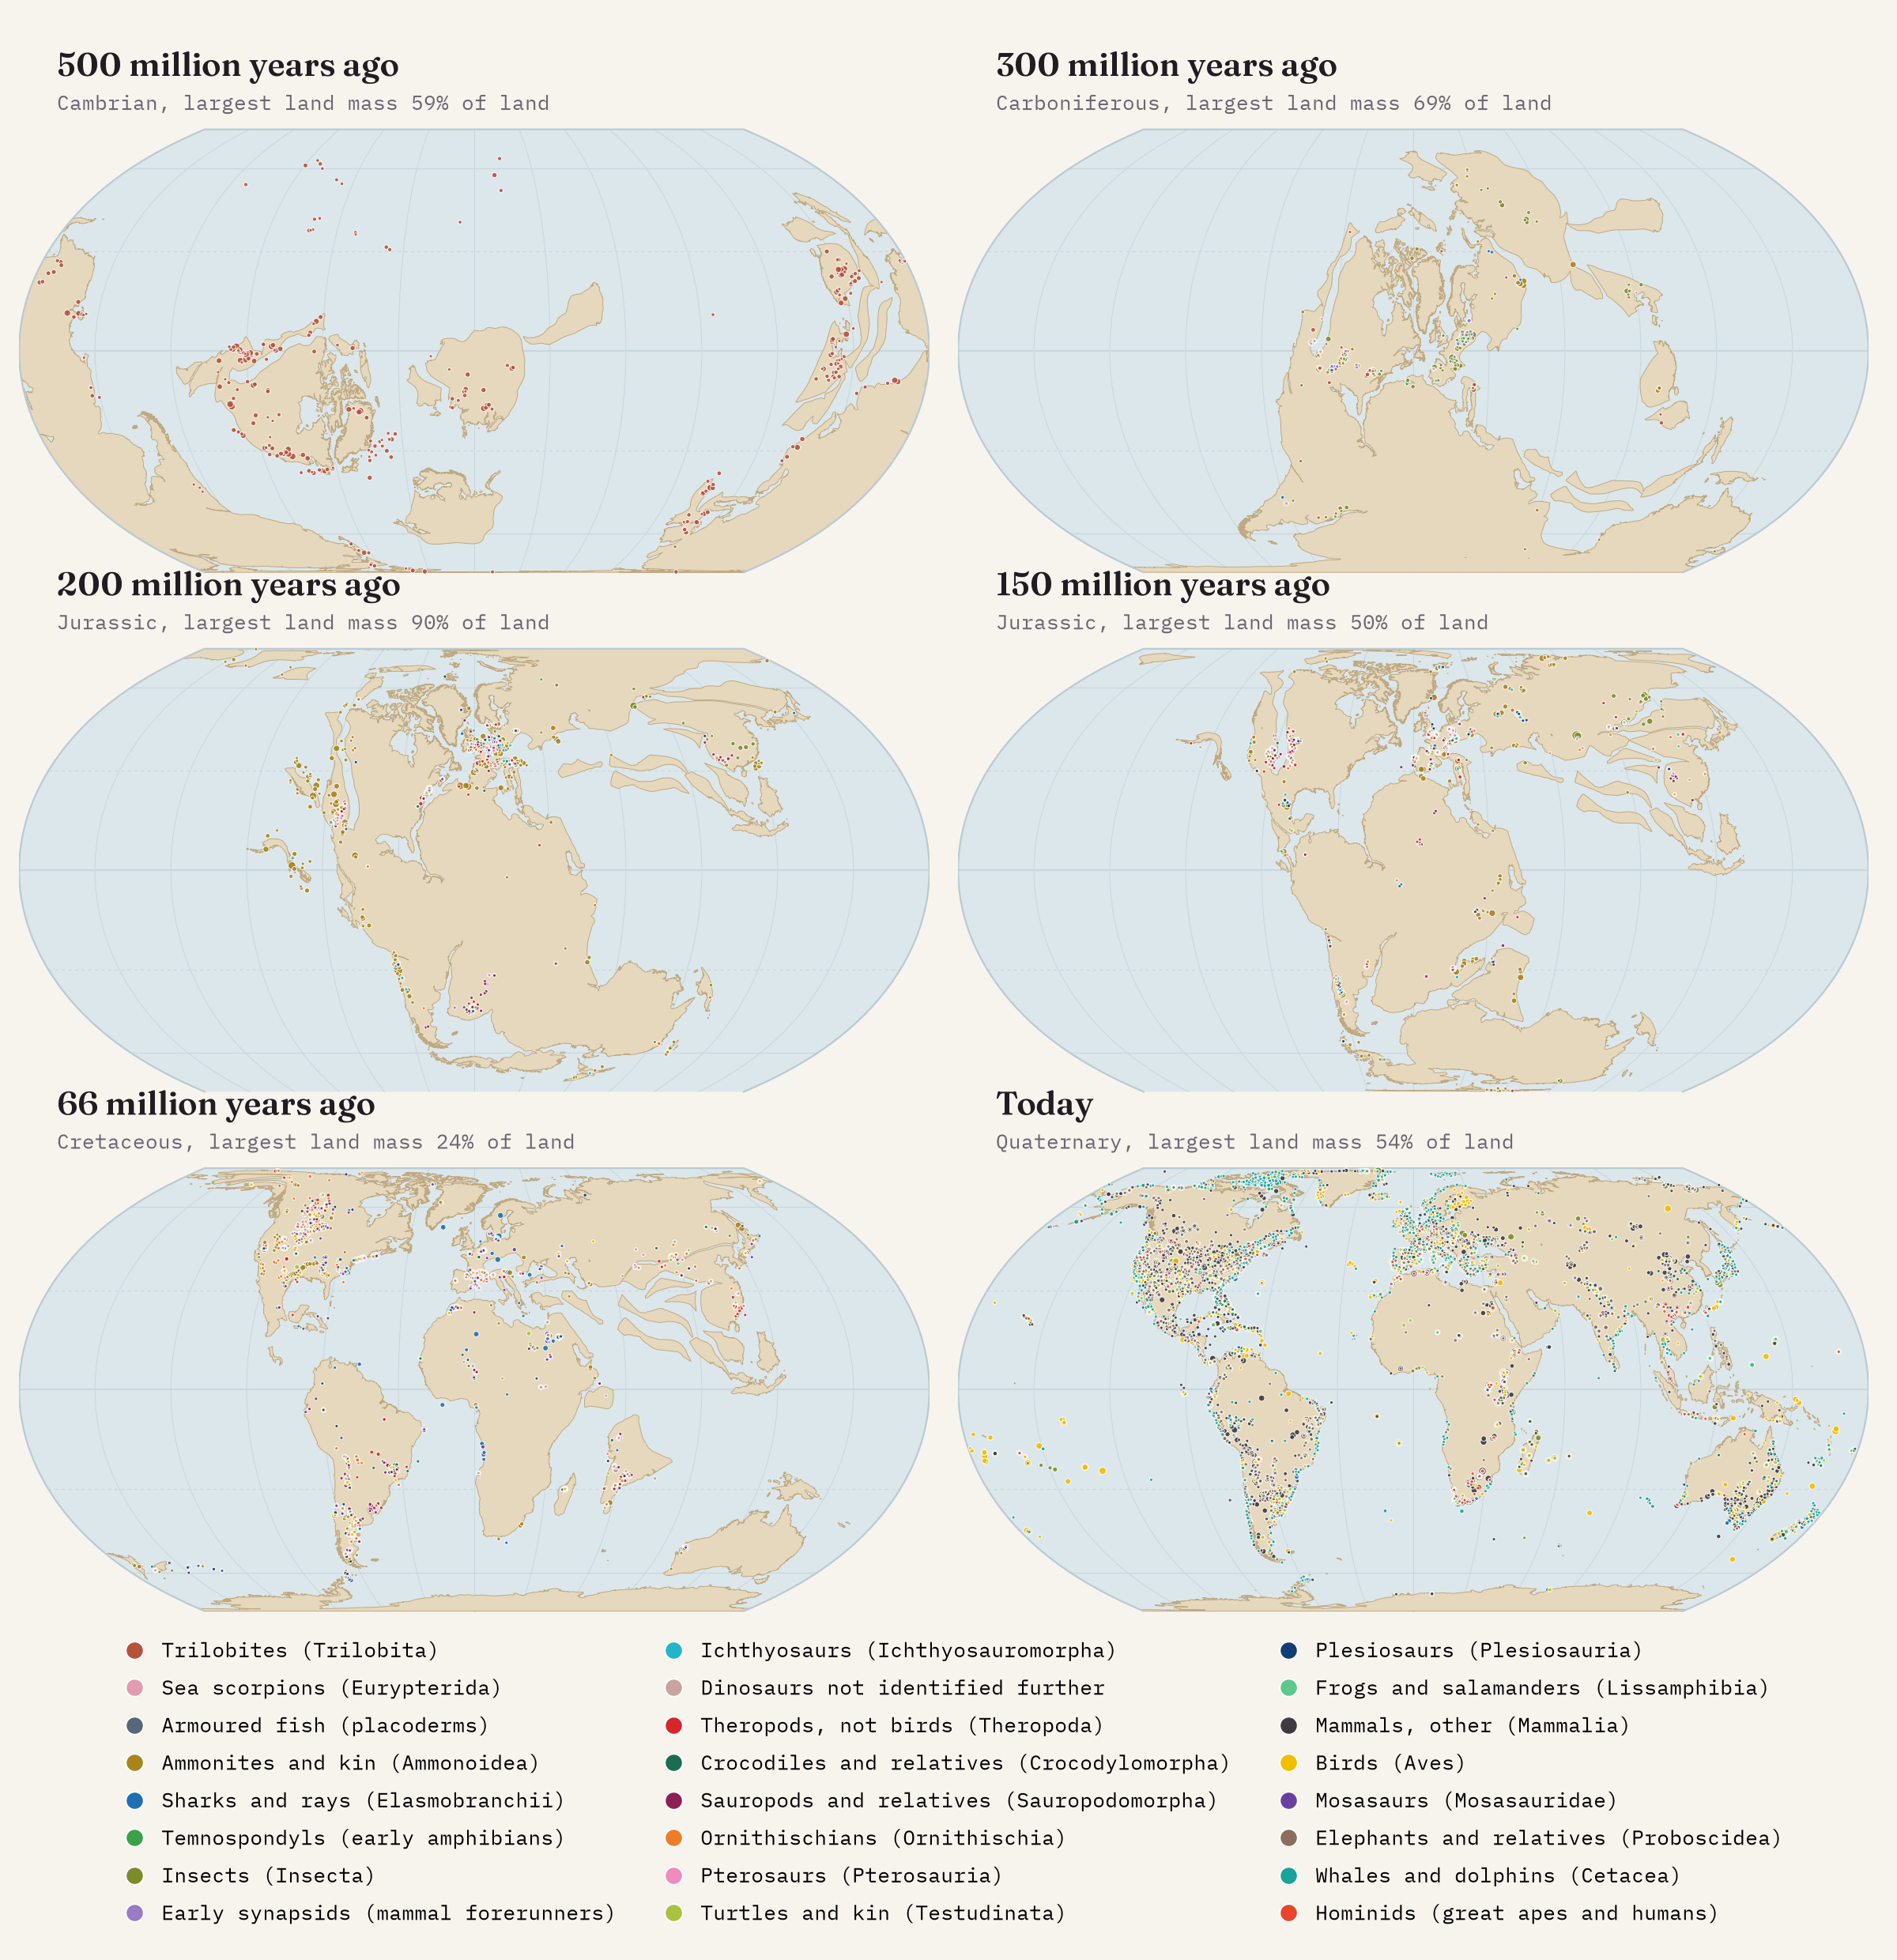
\includegraphics[width=\textwidth]{f_multiples.png}
\caption{Fossil occurrences at six ages, at their palaeo-positions on the PALEOMAP outlines, coloured by group. Each dot is a 1 degree cell; size grows with the number of occurrences.}\label{fig:multiples}\end{figure}

\begin{figure}[tbp]\centering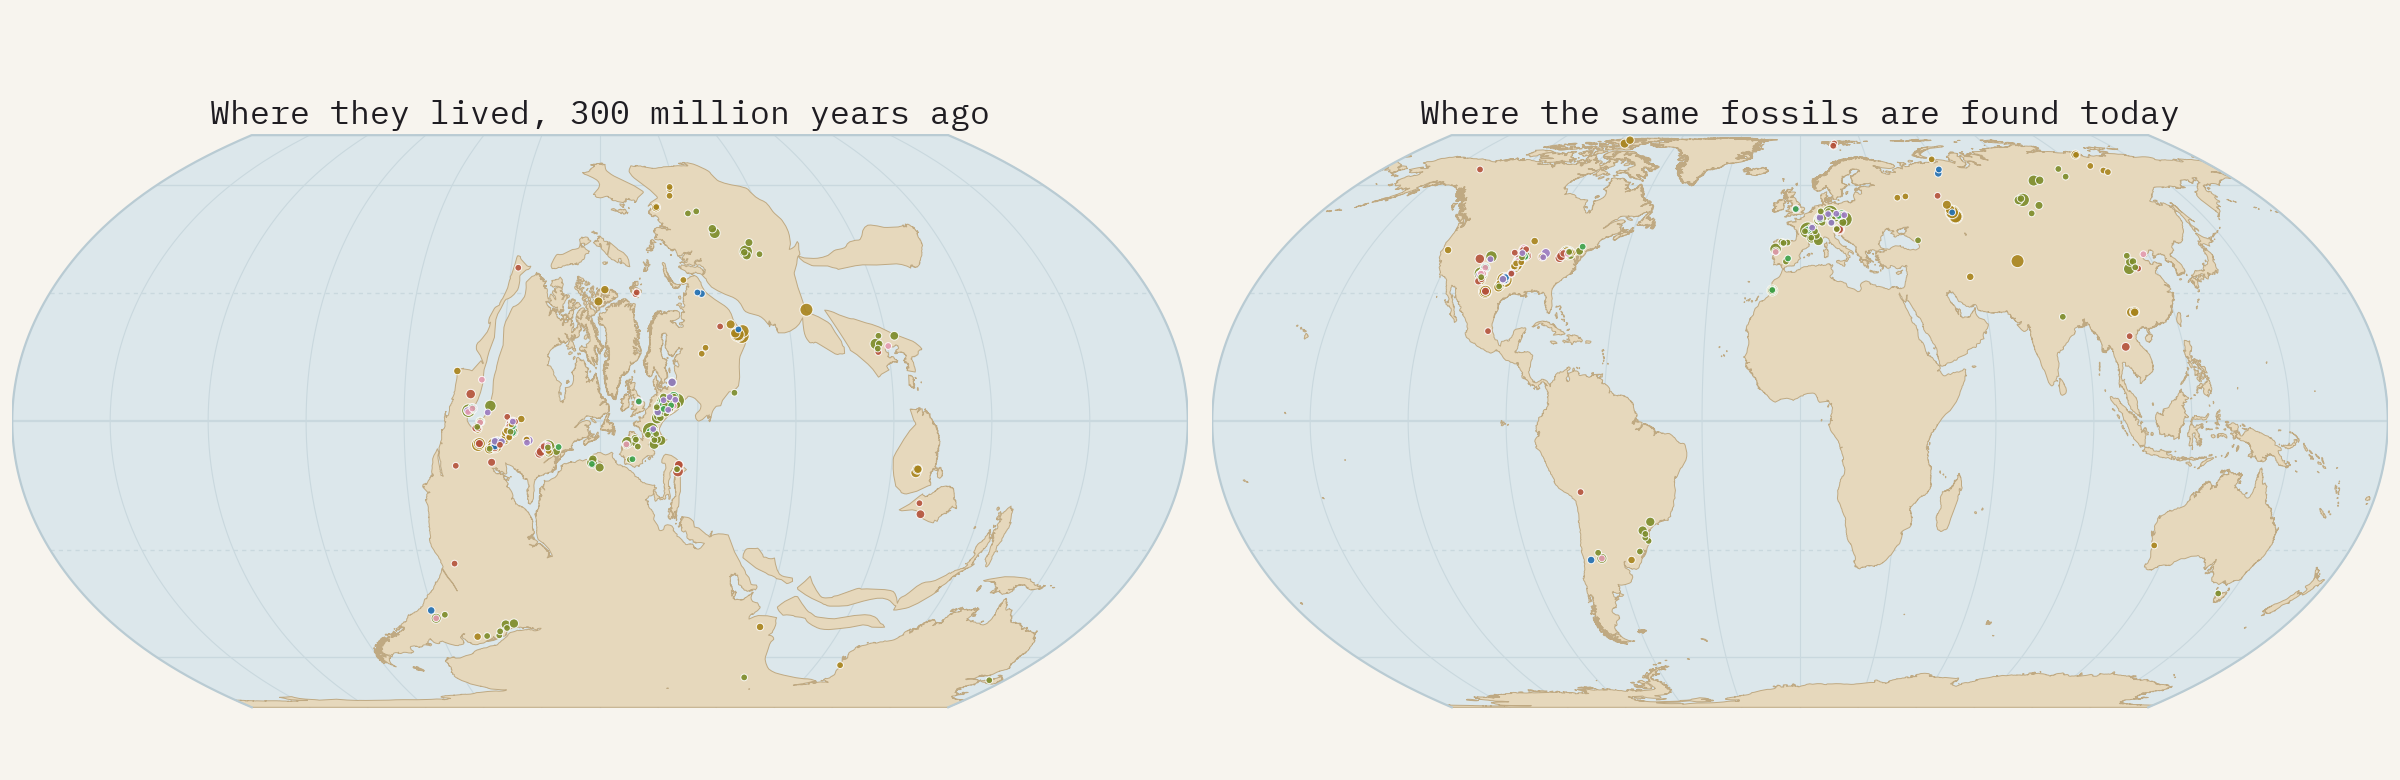
\includegraphics[width=\textwidth]{f_twoaddresses.png}
\caption{The same occurrences of 295 to 305 million years ago at their palaeo-positions (left) and present-day positions (right).}\label{fig:two}\end{figure}

\subsection{Pangaea}
The Pangaea index (Figure~\ref{fig:pangaea}) stays between 56 and 71\% from 540 to 280 million years ago, when Gondwana was the largest land mass. It rises in steps through the Carboniferous and Permian as the continents collide, reaching 87.9\% at 270 million years ago, stays above 85\% for 90 million years and peaks at 90.2\% at 180 million years ago. It then falls quickly: 72.4\% at 170, 50.1\% at 150 and 23.1\% at 100 million years ago. Today the largest land mass, Africa with Eurasia, holds 54.4\% of the land.

\begin{figure}[tbp]\centering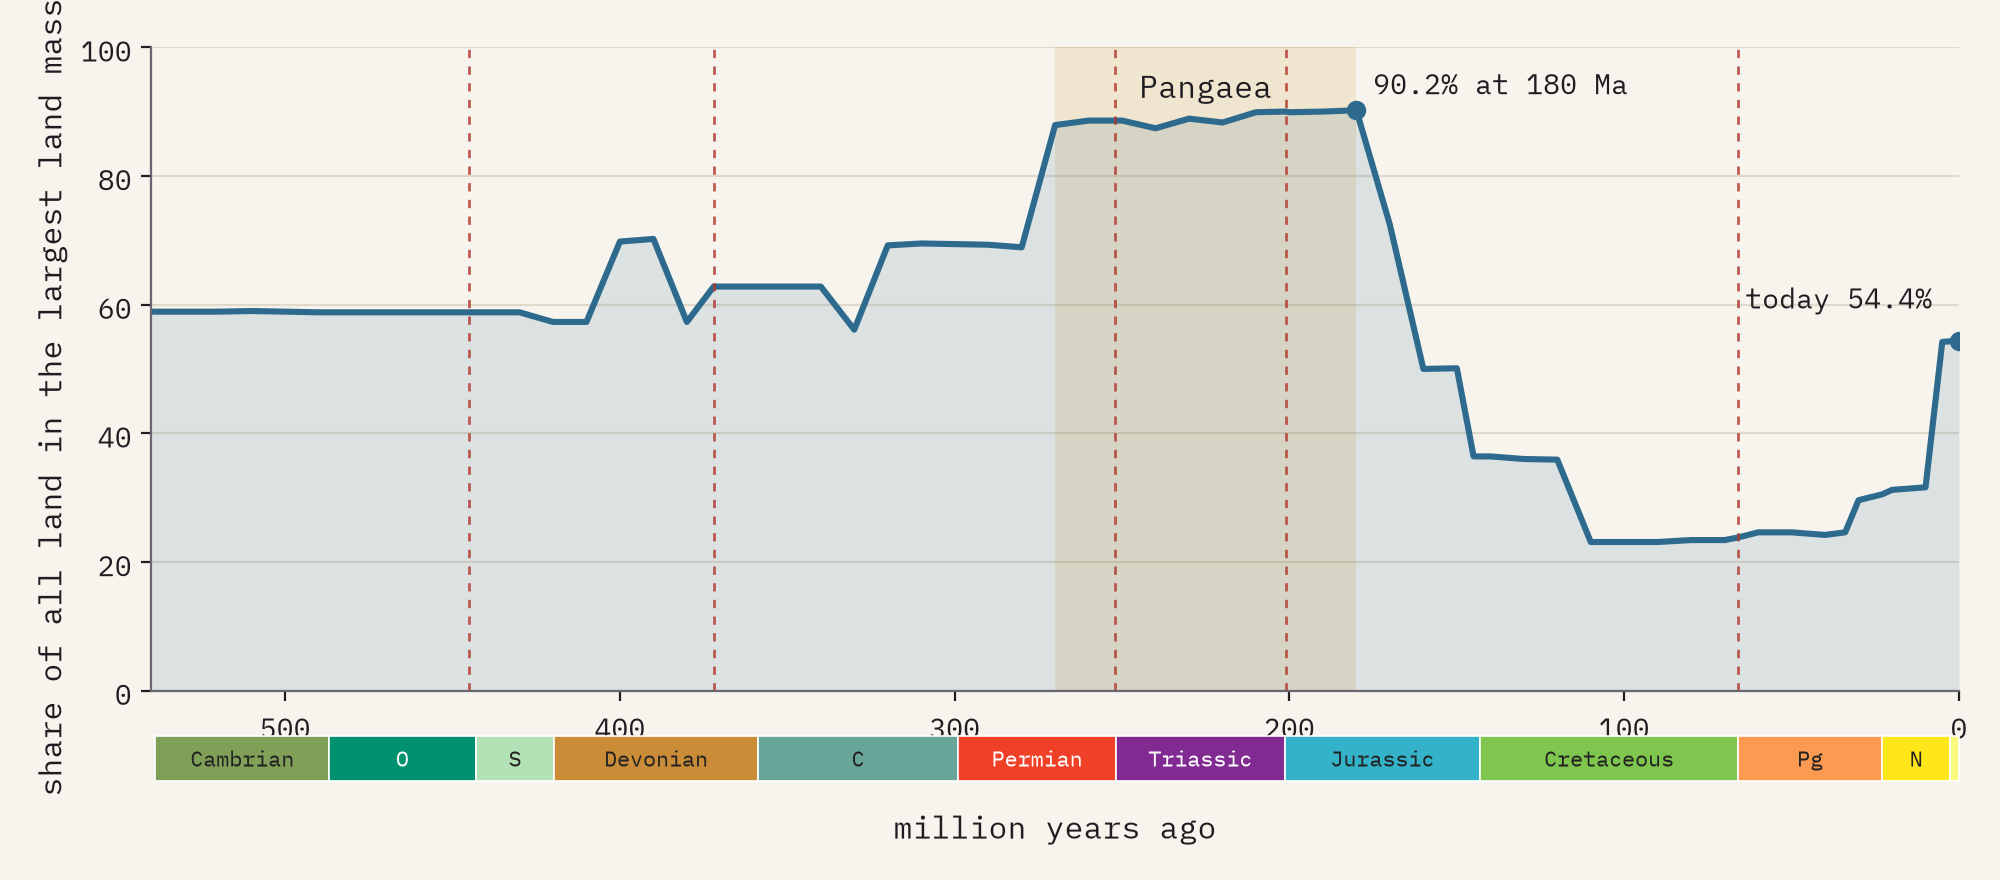
\includegraphics[width=.92\textwidth]{f_pangaea.png}
\caption{Pangaea index: share of all land in the largest connected land mass. Shaded: above 85\%. Dashed: the five mass extinctions.}\label{fig:pangaea}\end{figure}

\subsection{Which groups dominated the record}
Figure~\ref{fig:lanes} scales each group's genus counts to its own peak. The succession is familiar: trilobites and sea scorpions in the early Paleozoic, armoured fish in the Devonian, temnospondyls and synapsids in the late Paleozoic and Triassic, marine reptiles and dinosaurs in the Mesozoic, and mammals, whales, proboscideans and hominids in the Cenozoic. As a share of all genera in these groups, trilobites lead the Paleozoic (56.8\%), insects the Mesozoic (41.7\%) and mammals the Cenozoic (39.3\%). Insects have the most genera of any group (12,832), and their record is highly concentrated: the 50 richest of 5,580 insect collections hold 25.2\% of insect occurrences.

\begin{figure}[tbp]\centering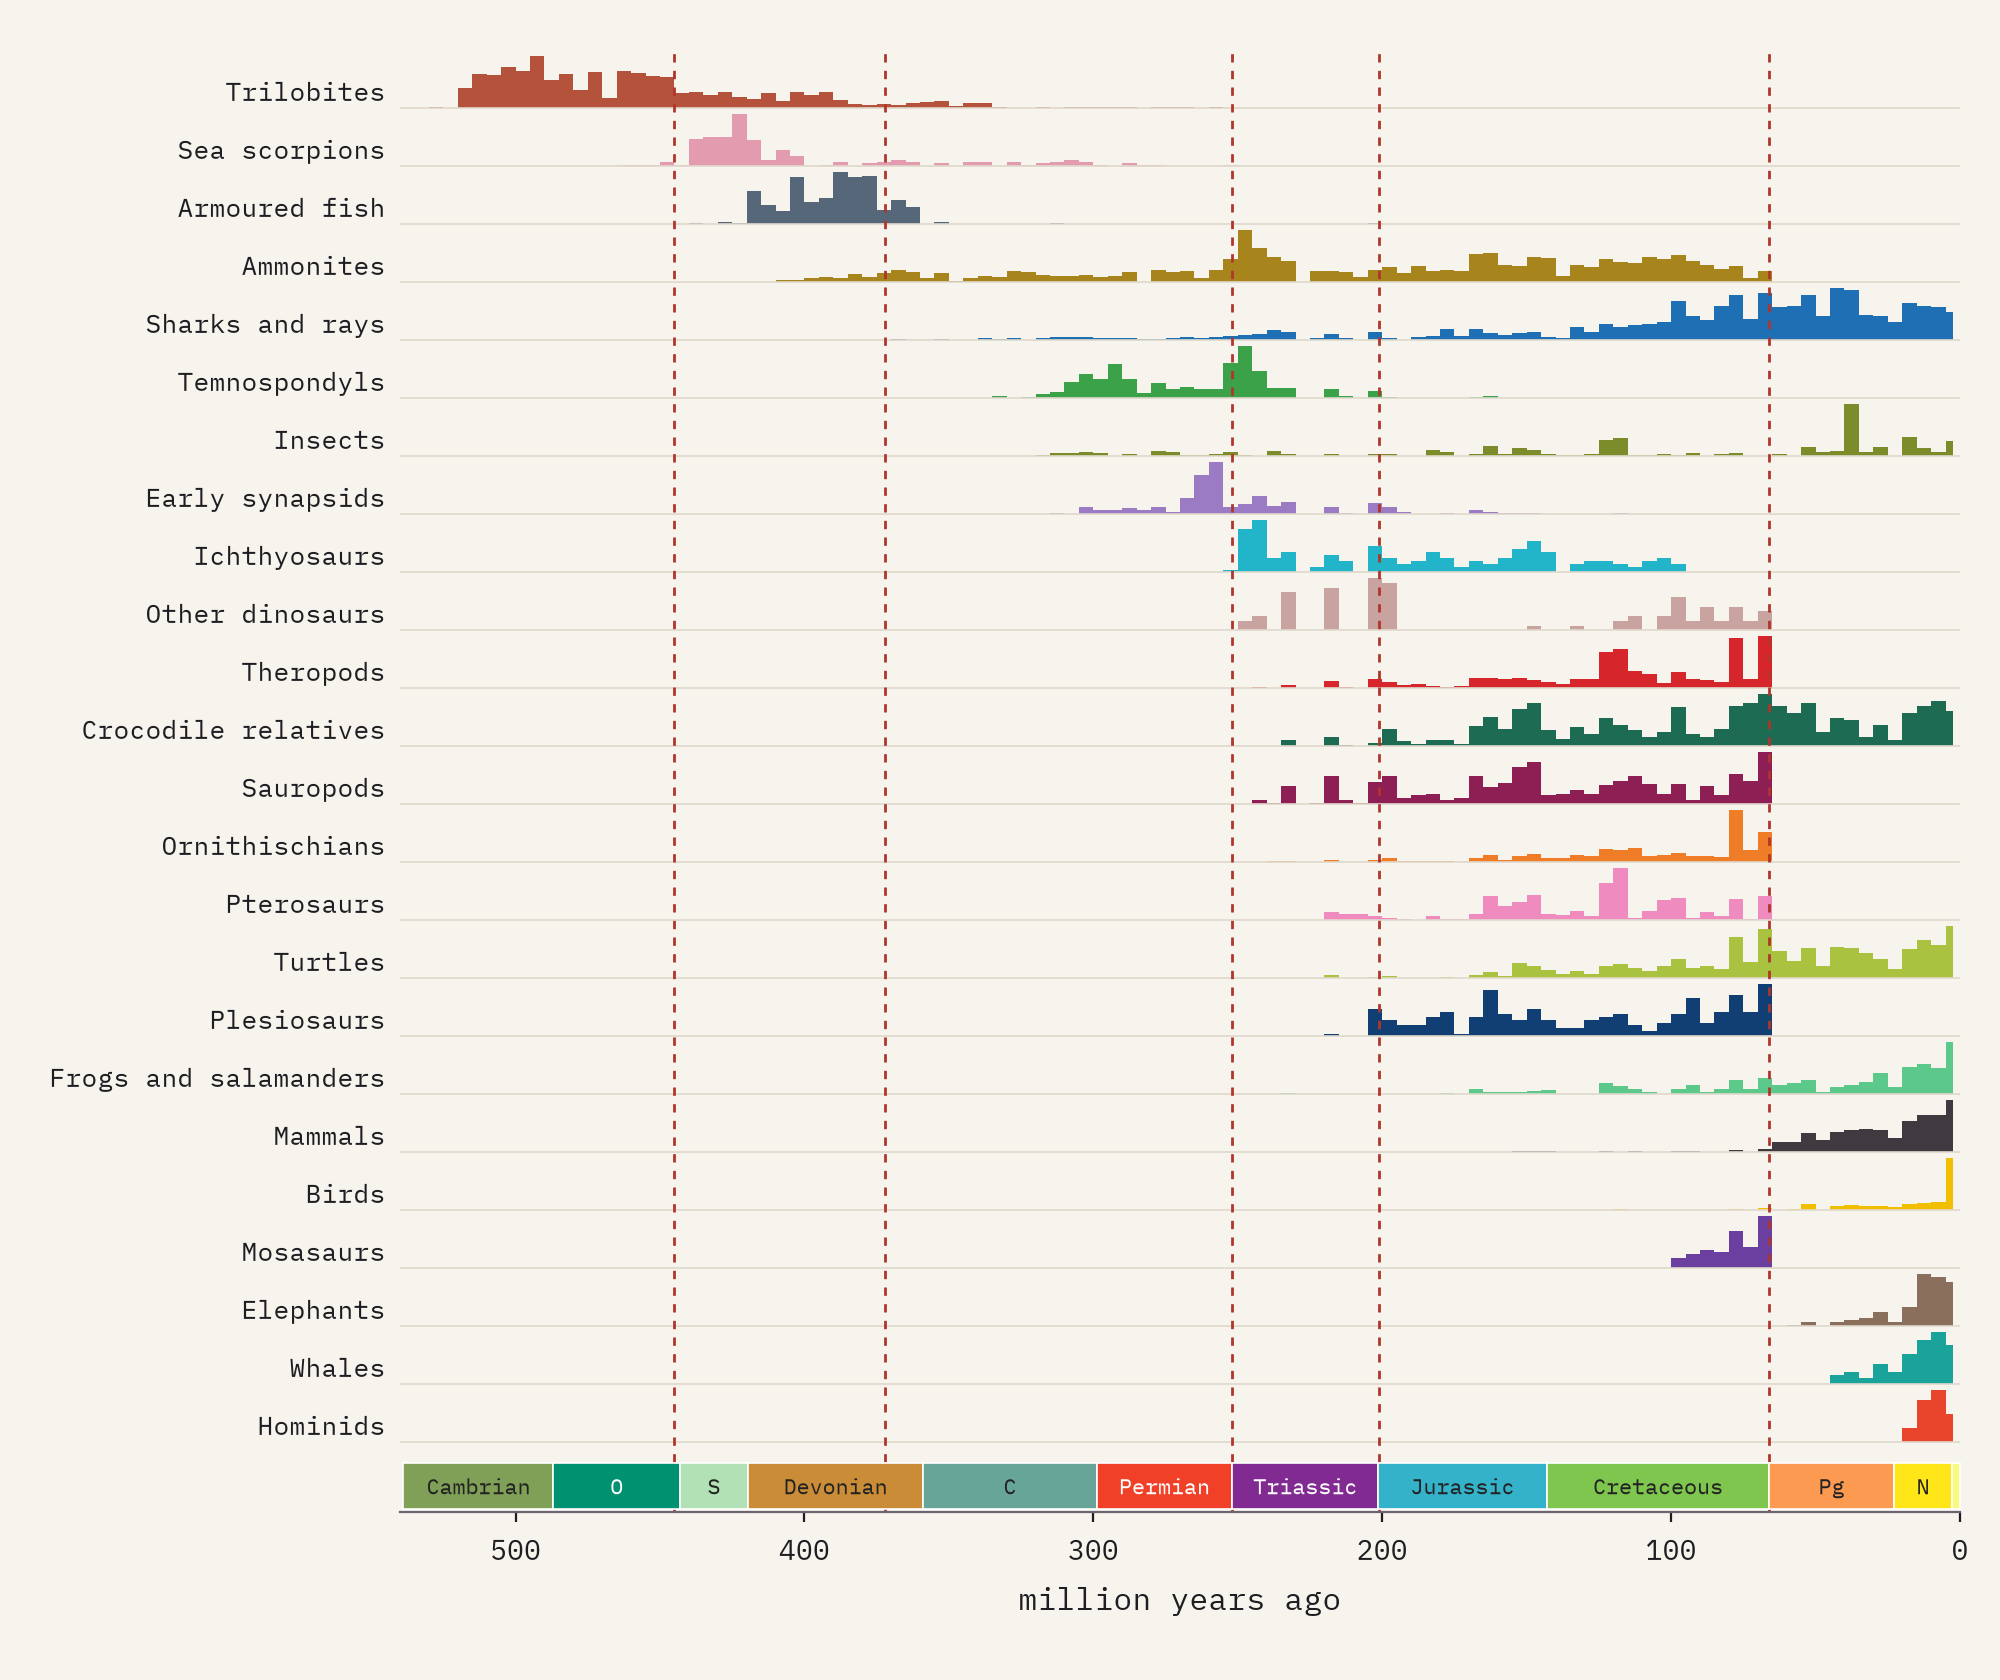
\includegraphics[width=.95\textwidth]{f_lanes.png}
\caption{Distinct genera per 5 million years for each group, each scaled to its own maximum. Groups in order of first appearance; dashed lines: mass extinctions.}\label{fig:lanes}\end{figure}

\subsection{Dinosaurs}
The data hold 20,231 occurrences of non-bird dinosaurs in 1,588 genera: 693 theropod, 380 sauropodomorph and 471 ornithischian genera. Genus counts are low through the Triassic and Jurassic and highest in the Late Cretaceous (Figure~\ref{fig:dinos}); the richest bin, 80 to 75 million years ago, has 316 genera, 75.0\% of its occurrences from North America. Of 203 genera from the Late Triassic and Early Jurassic, 11.3\% occur on two or more present-day continents, against 5.1\% of 1,180 Cretaceous genera (Figure~\ref{fig:cosmo}). The Late Jurassic stands out at 15.9\%, while the North Atlantic was still narrow. All tyrannosaurid and ceratopsid occurrences are from North America, Asia or Europe; 88.1\% of abelisaurid occurrences are from the southern continents and India. 245 dinosaur collections lie beyond 60 degrees of palaeo-latitude and 53 beyond 75 degrees, chiefly in Alaska and Victoria, Australia.

\begin{figure}[tbp]\centering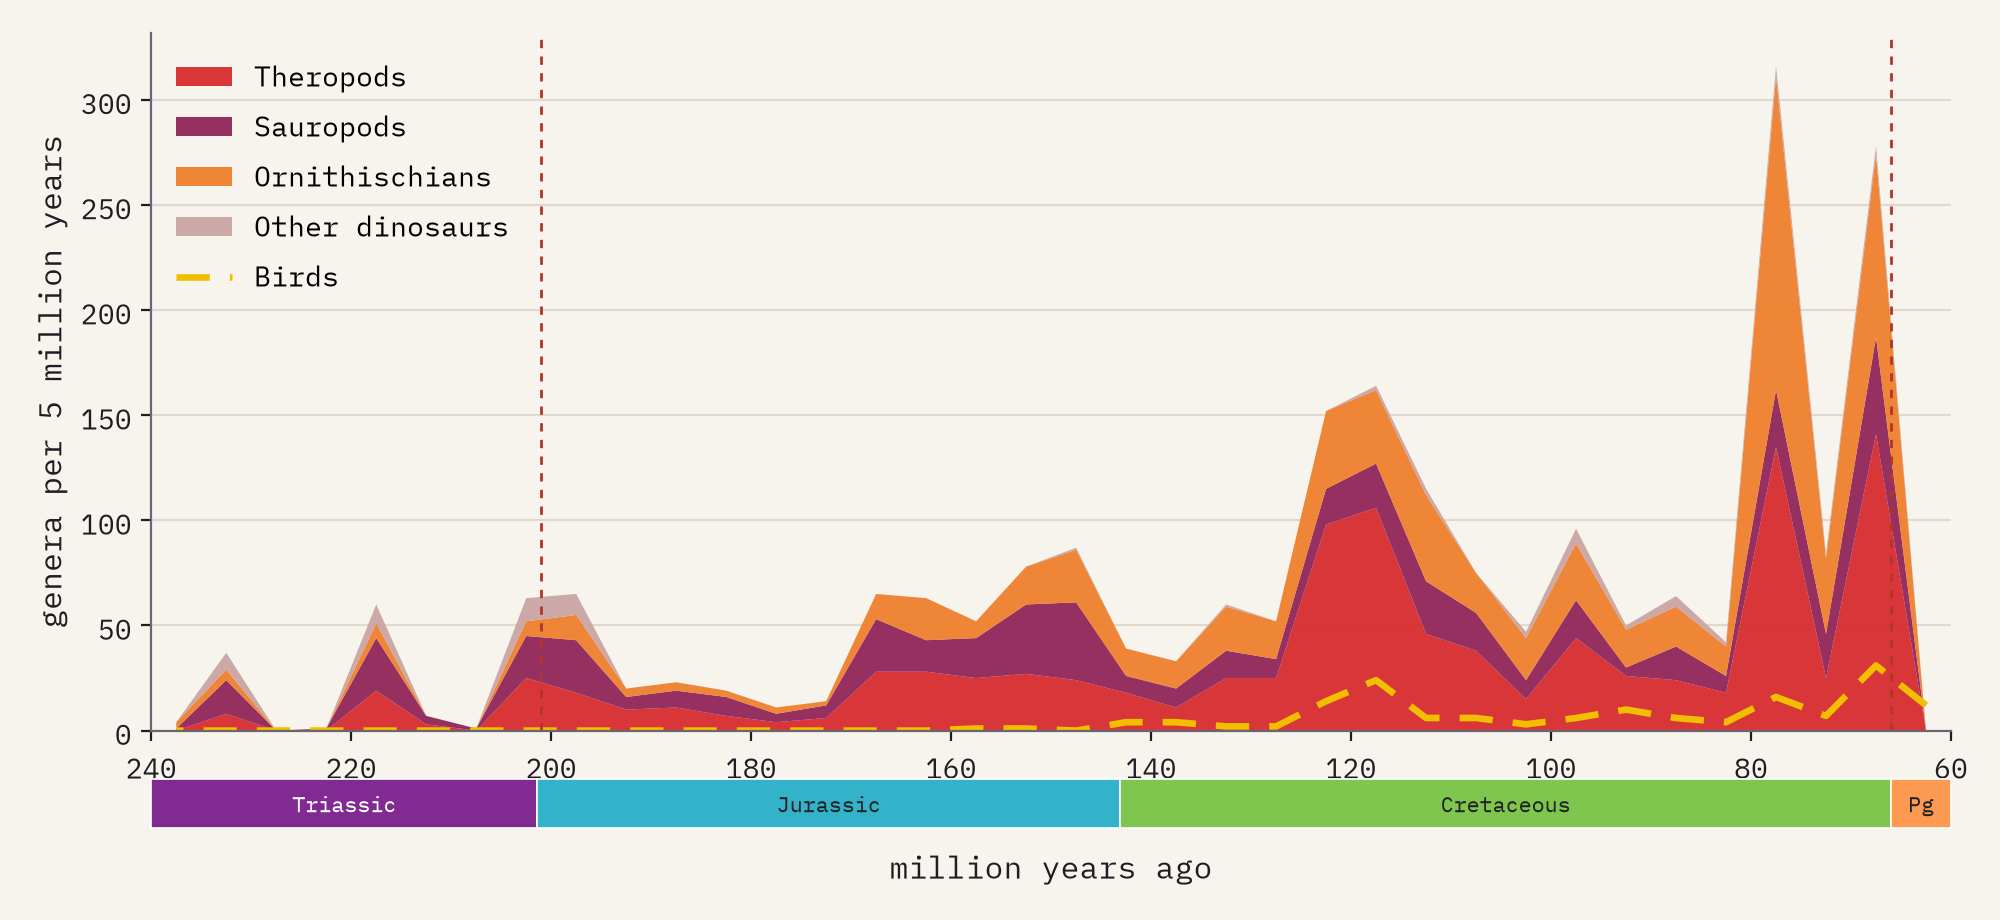
\includegraphics[width=.92\textwidth]{f_dinos.png}
\caption{Dinosaur genera per 5 million years, stacked by group, with birds as a dashed line.}\label{fig:dinos}\end{figure}

\begin{figure}[tbp]\centering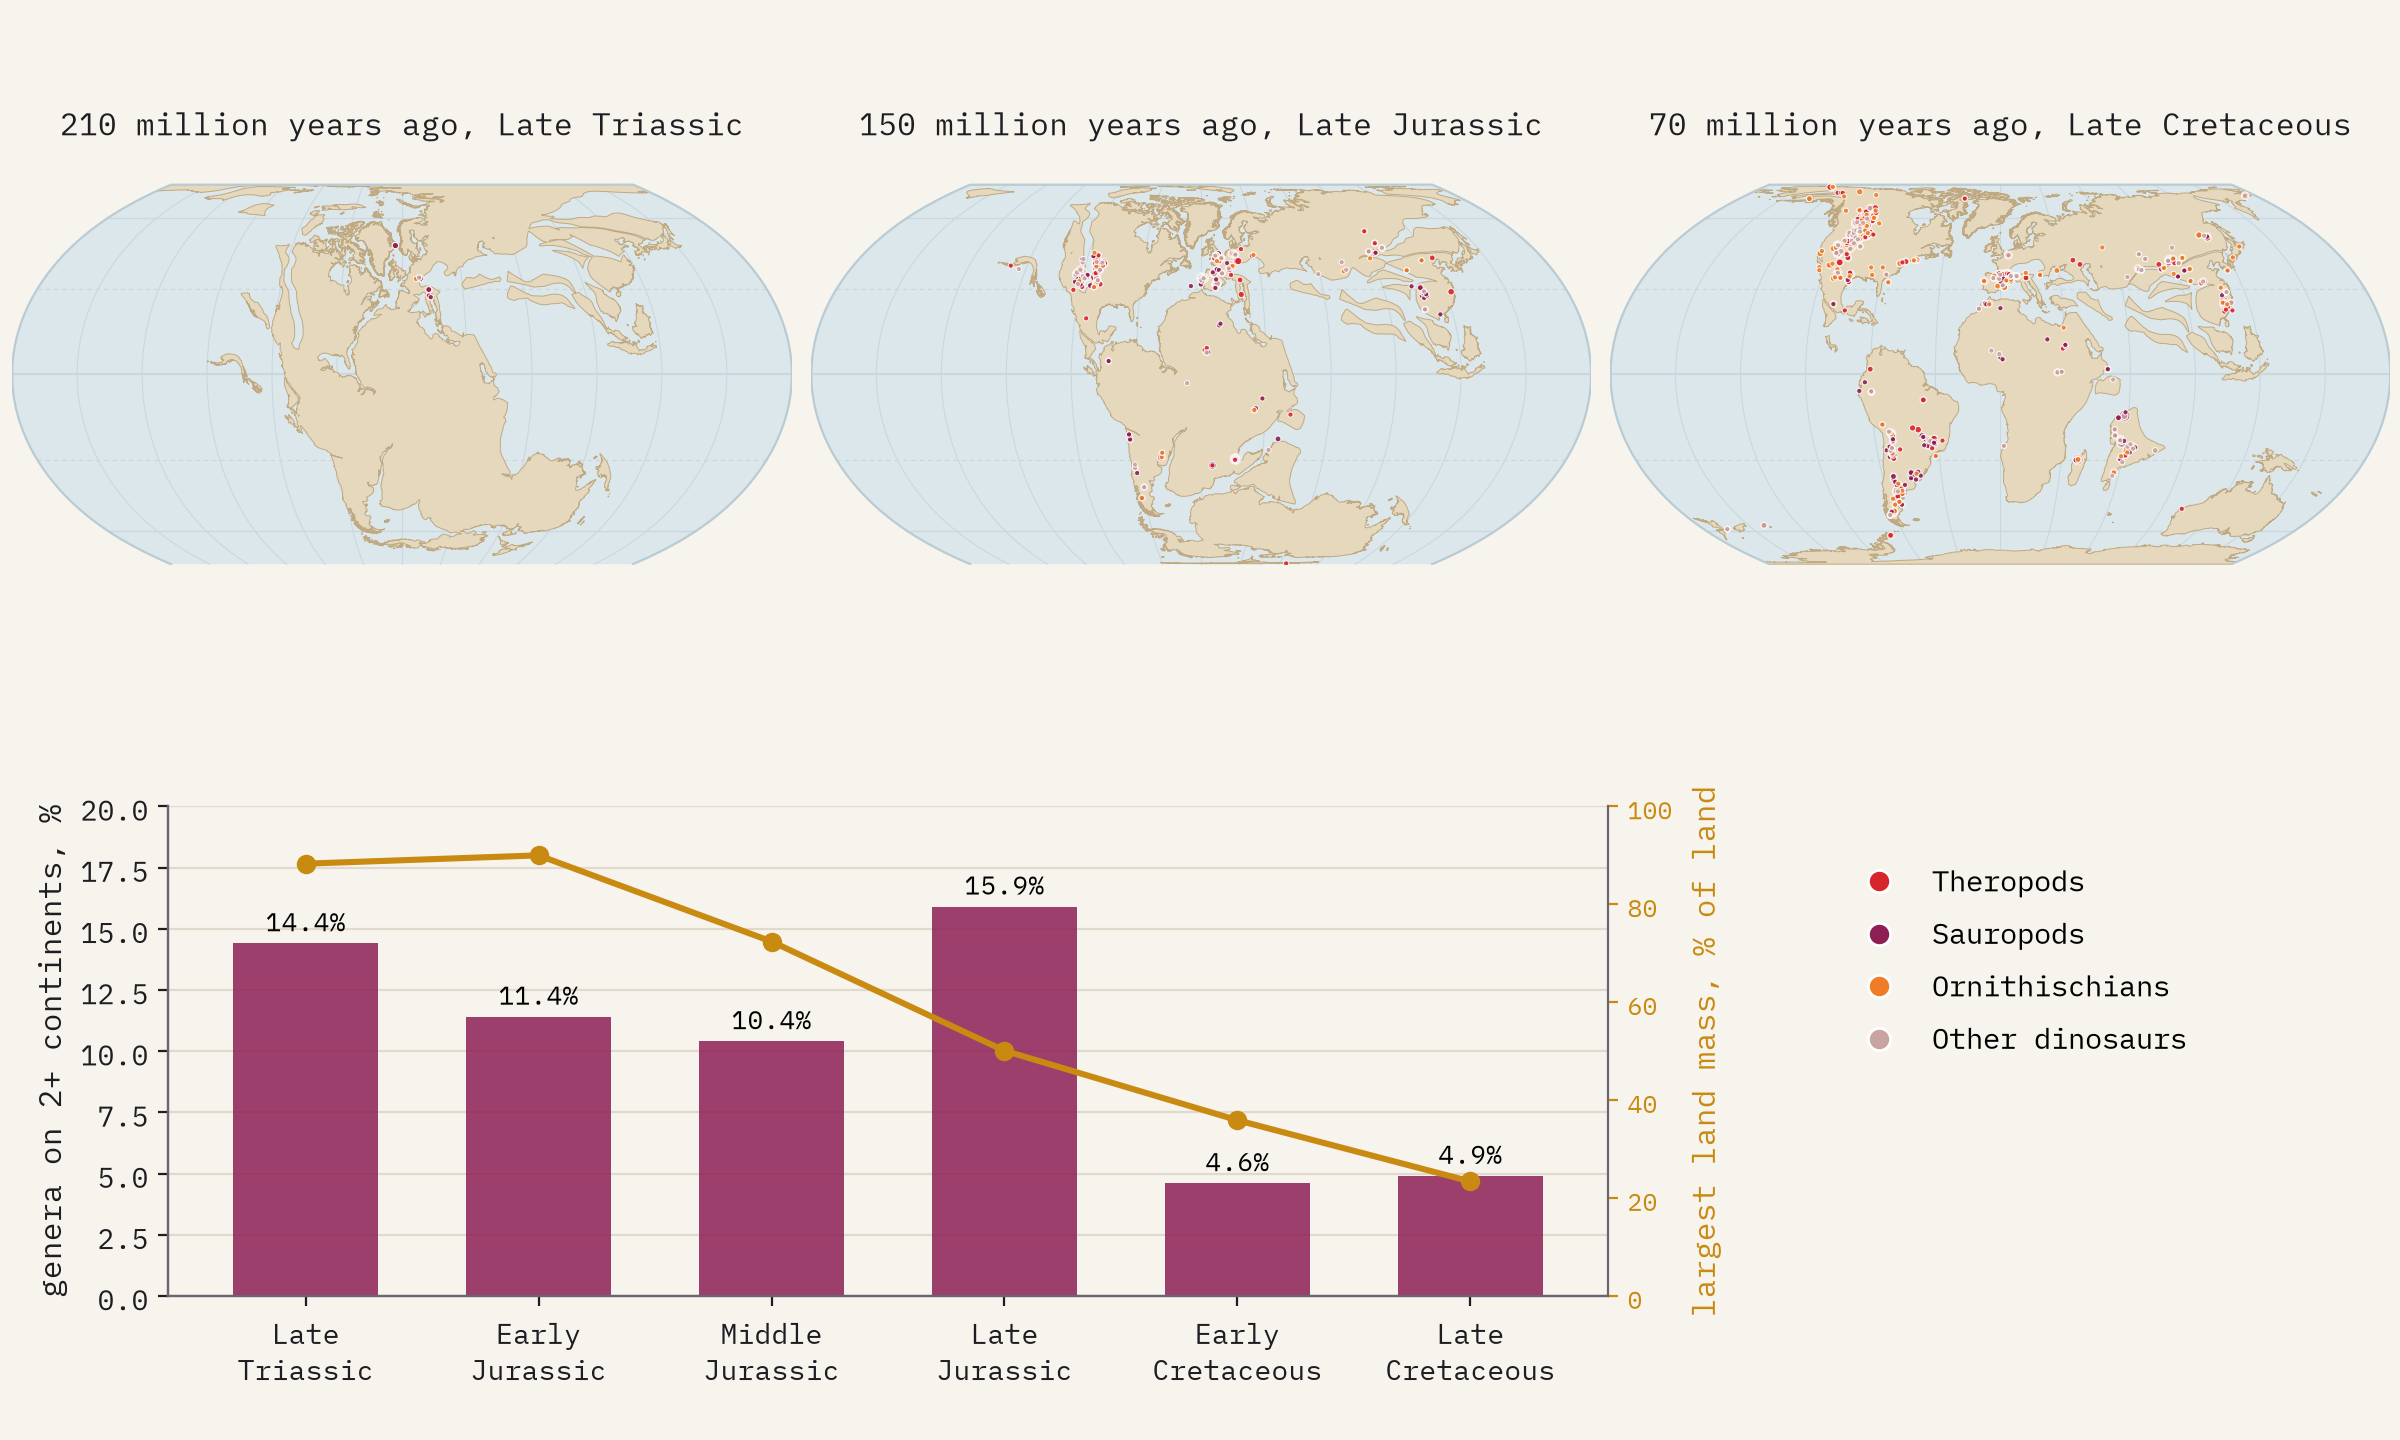
\includegraphics[width=\textwidth]{f_cosmo.png}
\caption{Top: non-bird dinosaur occurrences at 210, 150 and 70 million years ago. Bottom: share of genera in each interval found on two or more present-day continents (bars) and the Pangaea index at the nearest outline age (line).}\label{fig:cosmo}\end{figure}

\subsection{Latitude}
Median absolute palaeo-latitudes range from 8.5 degrees for hominids to 48.4 degrees for non-mammal synapsids (Figure~\ref{fig:lat}). Trilobite collections have a median of 19.8 degrees, ammonoids 32.8 and theropods 37.4. Because most collections come from the Northern Hemisphere continents, which have been studied most, latitudinal spreads describe the record rather than the full ranges of the animals.

\begin{figure}[tbp]\centering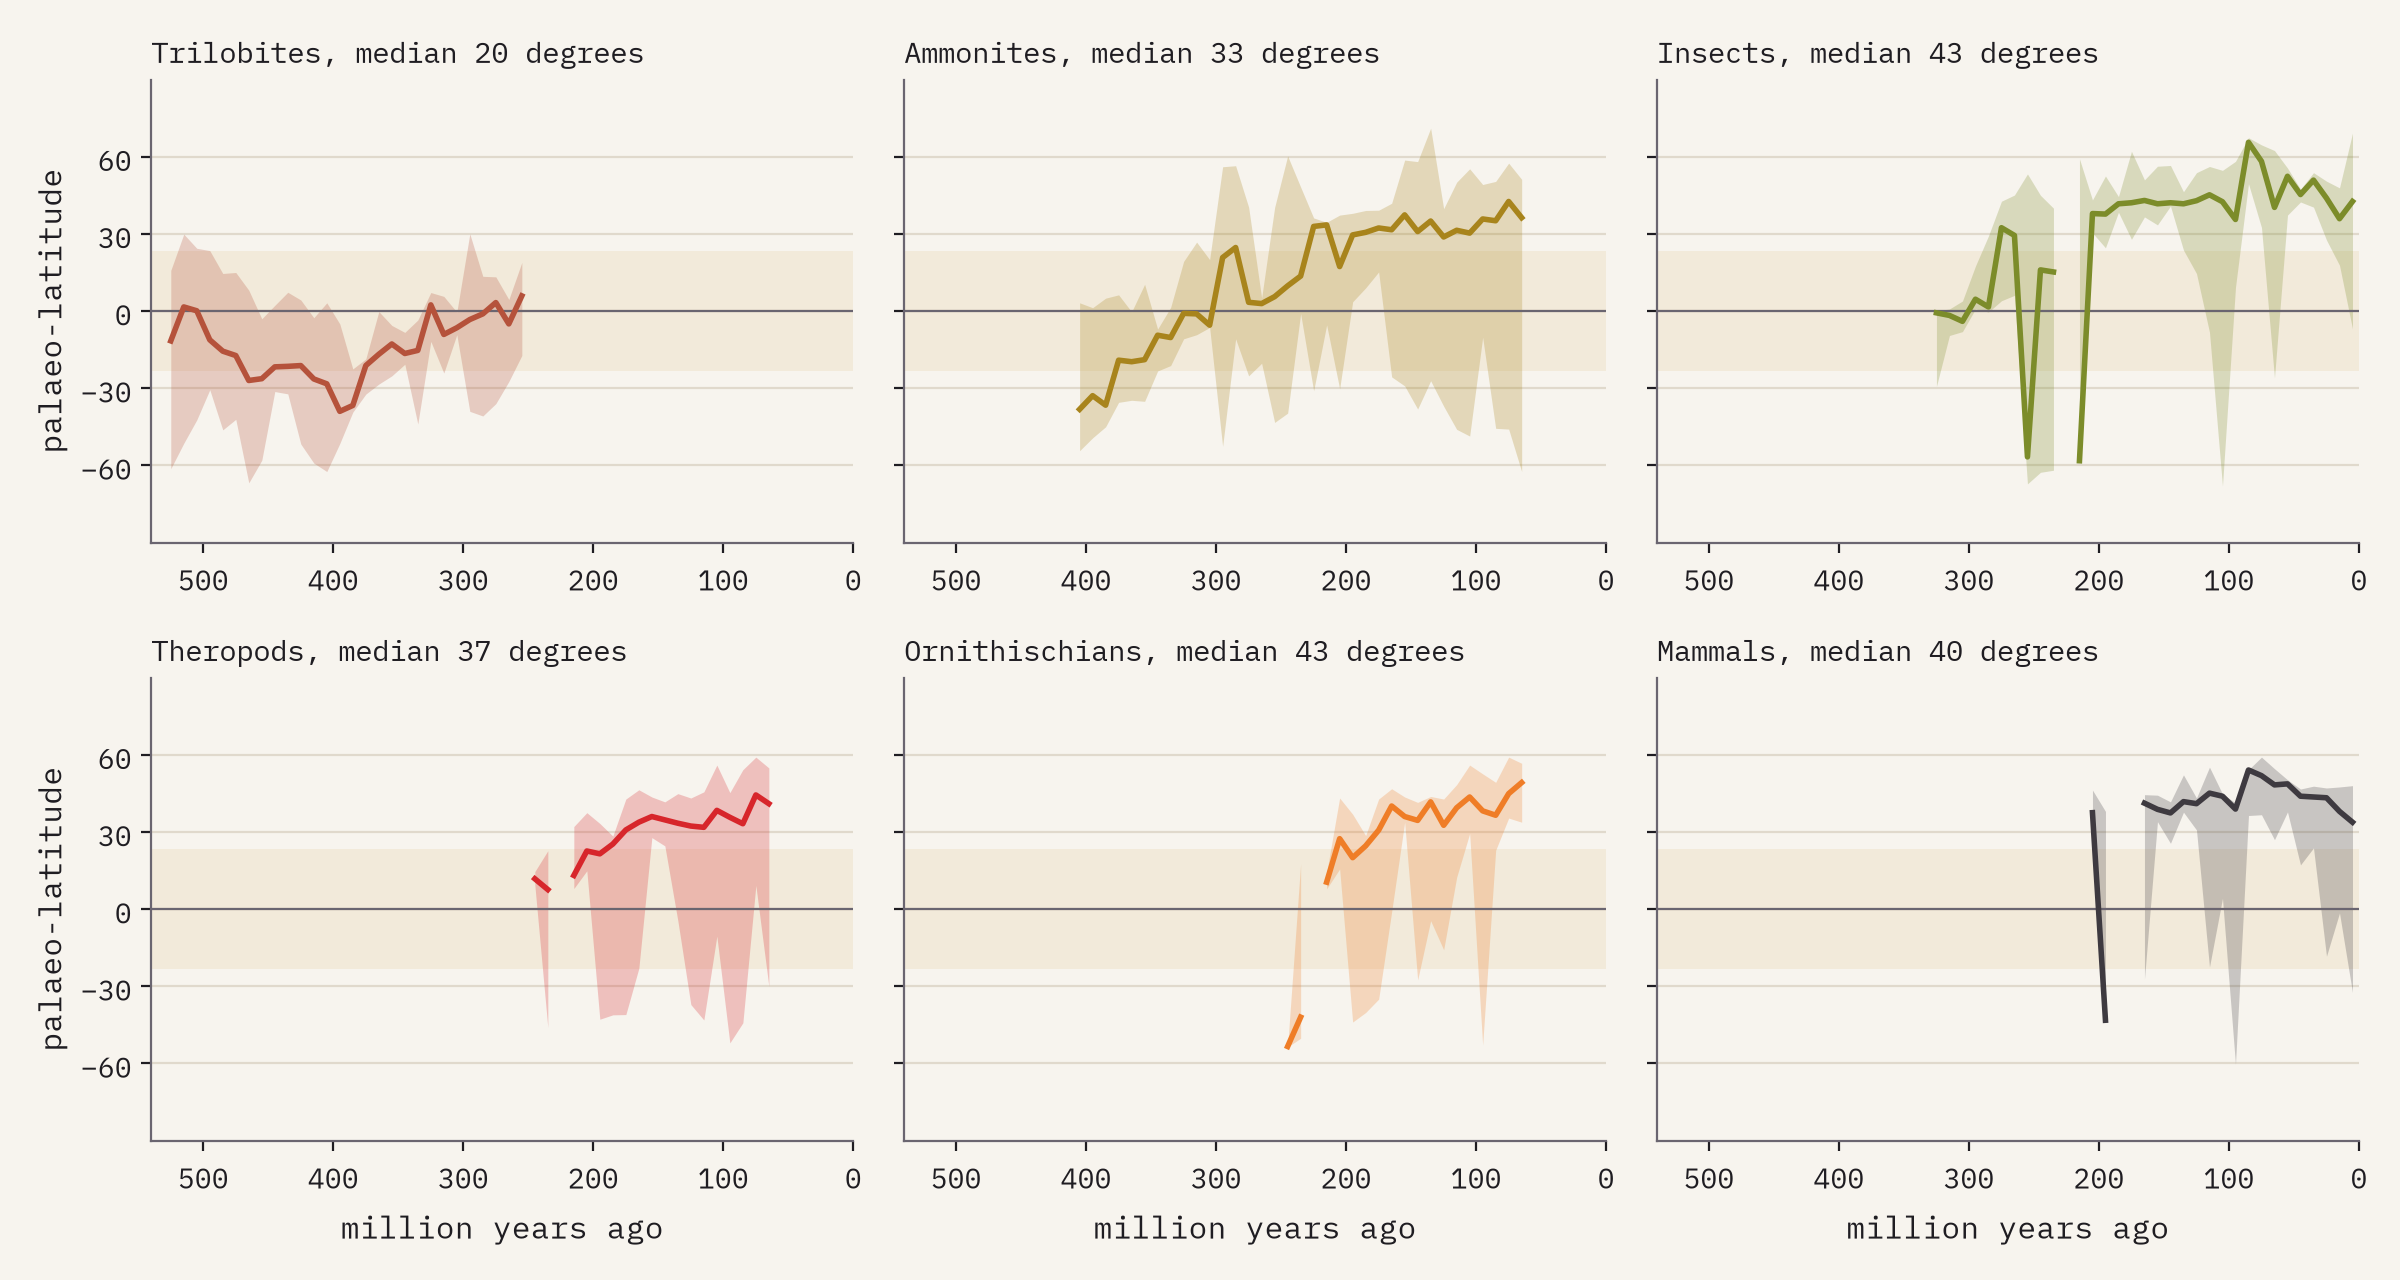
\includegraphics[width=\textwidth]{f_latitude.png}
\caption{Palaeo-latitude of collections by 10 million year step for six groups: median (line) and 10th to 90th percentiles (band). Shaded: the tropics.}\label{fig:lat}\end{figure}

\subsection{Mass extinctions}
Figure~\ref{fig:ext} shows the last-appearance measure at the five extinctions. The end-Permian is the highest (74.4\% of 414 genera), above the 90th percentile of the background. The end-Ordovician (61.6\%), Late Devonian (60.9\%) and end-Cretaceous (56.7\%) are well above the background median; the end-Triassic (33.2\%) is not, probably because much of its toll fell on groups not included here and because Late Triassic sampling is thin. At the end-Cretaceous every genus of non-bird dinosaur, plesiosaur and mosasaur with at least two collections is last seen before the boundary, as are 97.1\% of ammonoids, against 1.5\% of insects.

\begin{figure}[tbp]\centering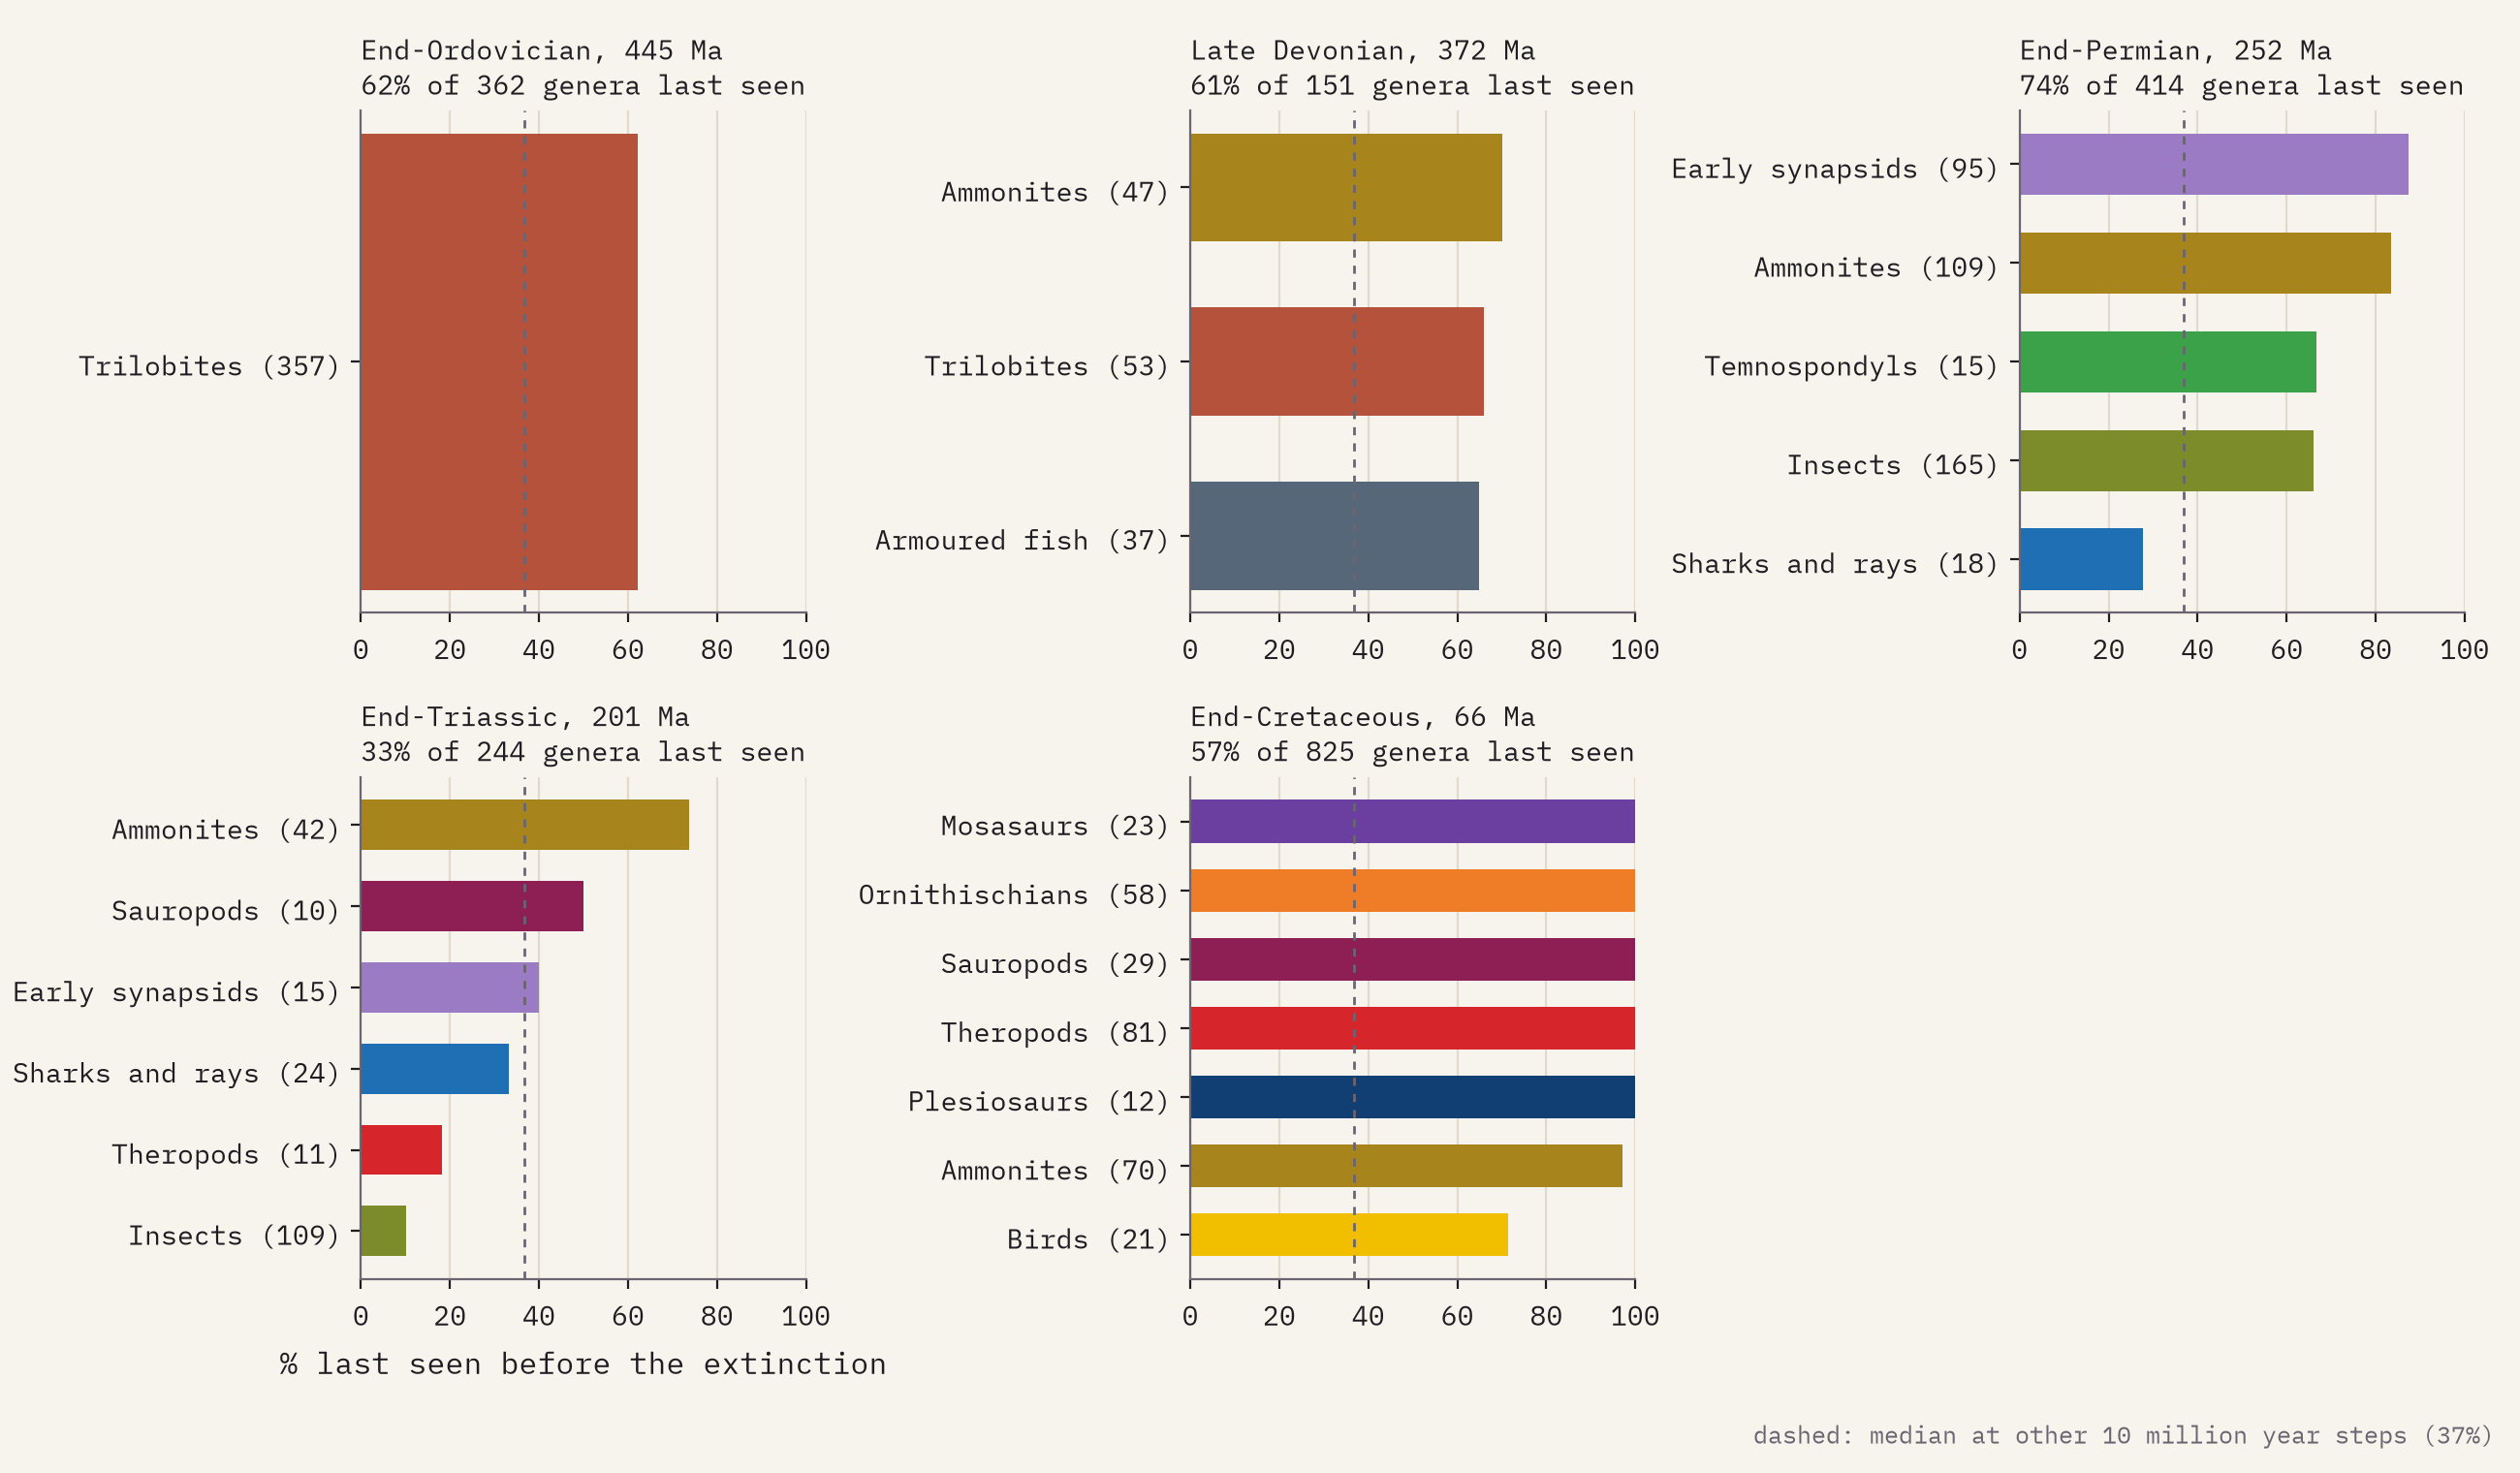
\includegraphics[width=\textwidth]{f_extinctions.png}
\caption{Share of standing genera (with at least two collections) last seen in the 10 million years before each extinction, by group (groups with at least 10 standing genera; number standing in brackets). Dashed: median of the same measure at other 10 million year steps.}\label{fig:ext}\end{figure}

\subsection{Sampling}
North America holds 35.7\% of occurrences and Europe 29.9\%; together 65.6\%, against 32.2\% of the land area. The United States alone has 27.7\%; Africa 8.5\% and South America 6.5\% (Figure~\ref{fig:samp}). The North American and European share is similar in each era (Paleozoic 67.0\%, Mesozoic 62.4\%, Cenozoic 67.4\%) but swings widely between 5 million year bins.

\begin{figure}[tbp]\centering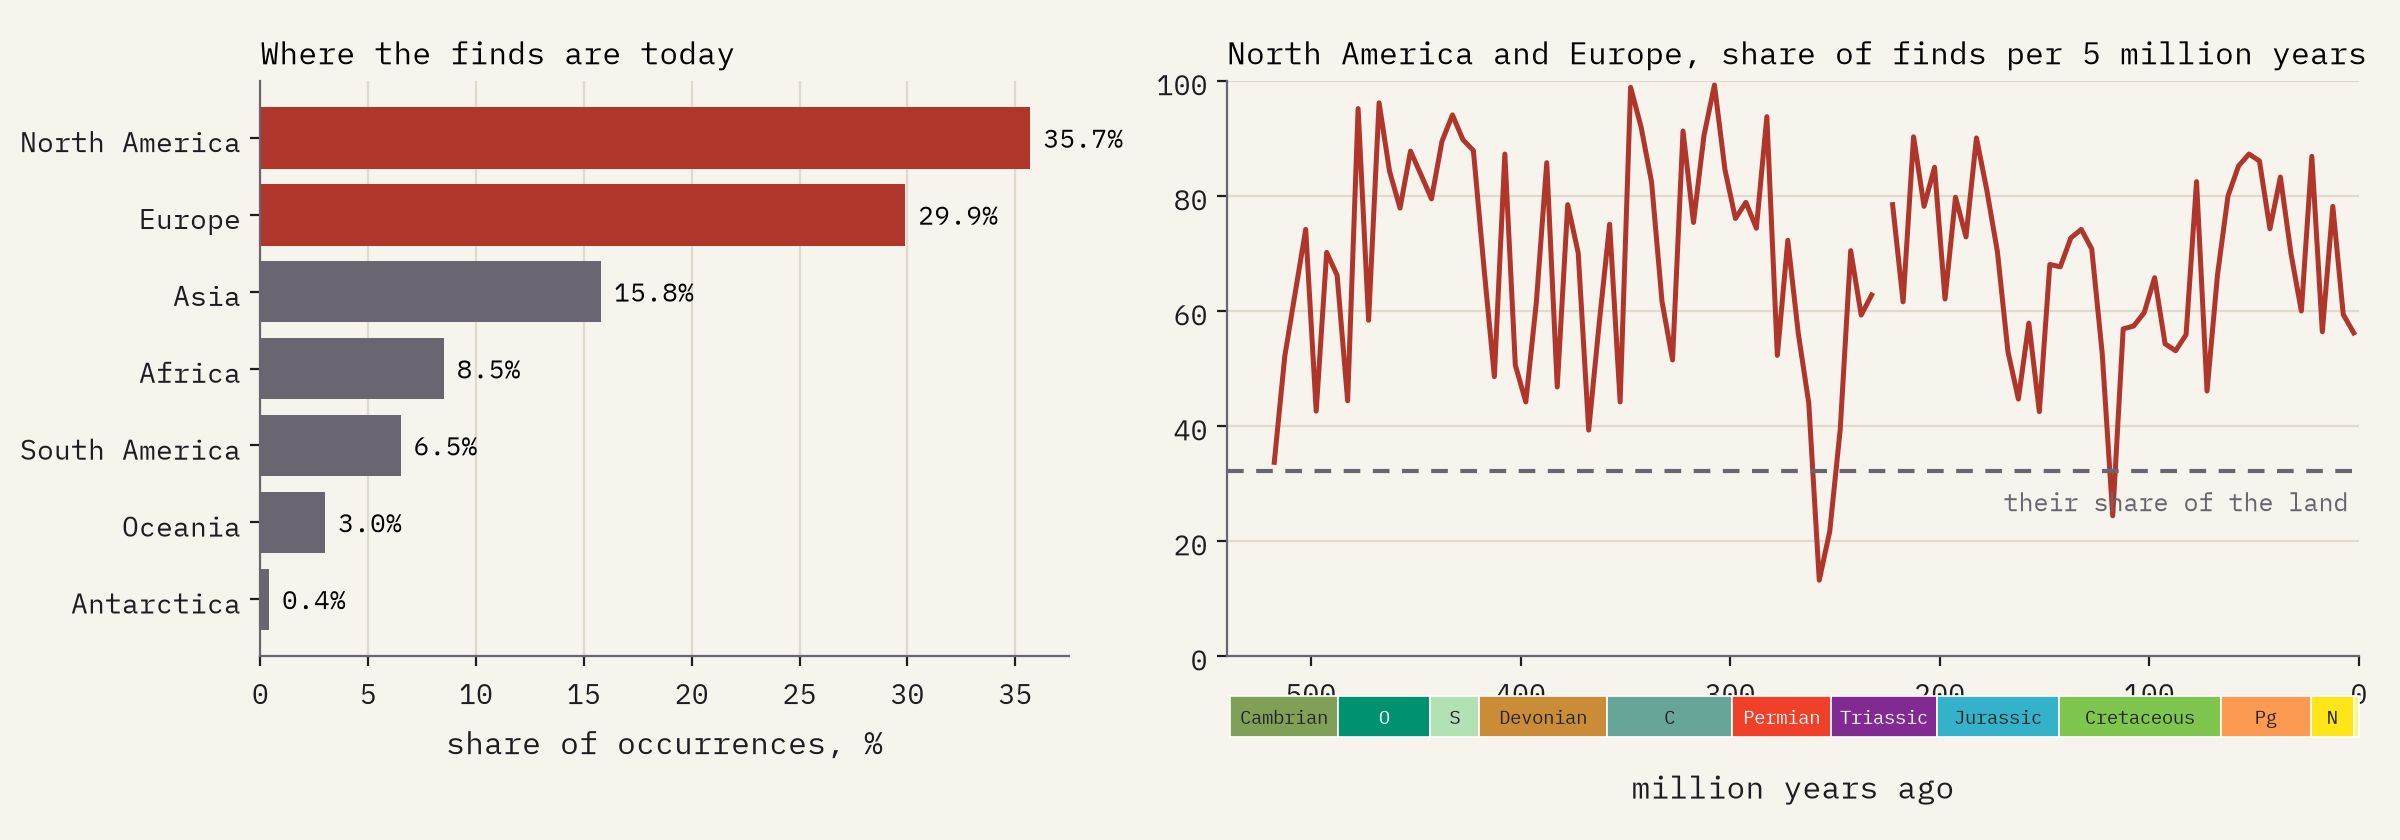
\includegraphics[width=\textwidth]{f_sampling.png}
\caption{Left: occurrences by present-day continent. Right: share of occurrences from North America and Europe per 5 million years (bins with at least 20 collections); dashed, their share of today's land.}\label{fig:samp}\end{figure}

\section{Discussion}
Placed at their ancient positions, open fossil data reproduce the broad textbook picture of the Phanerozoic: the dominance of trilobites in early Paleozoic seas, the assembly and break-up of Pangaea, the provincial faunas of the Cretaceous, and the turnover at the great extinctions. That such a picture emerges from simple counts is a tribute to the decades of work collected in the Paleobiology Database. But each pattern is also a pattern of sampling. Genus counts follow the area of exposed rock of each age and the effort spent on it \citep{raup1972,smith2007,alroy2008}; the high Late Cretaceous dinosaur counts reflect, in part, the badlands of western North America; and the latitudinal patterns reflect the positions of the well-studied Northern Hemisphere continents. The cosmopolitanism result fits the expectation that faunas became more provincial as Pangaea broke up \citep{brusatte2015}, but genus definitions and national traditions of naming add noise that this simple measure cannot remove.

\section{Limitations}
First, occurrence counts are not abundance, and genus counts are not true diversity: no correction for sampling is applied. Second, ages are midpoints of often long ranges, so the timing of events is blurred by several million years, and bins fill unevenly. Third, palaeo-positions come from one plate model at each collection's own age; other models differ, uncertainty grows with age, and map dots can sit up to 5 million years away from the outline age. Fourth, the outlines are present-day coastlines and blocks moved in time, not ancient shorelines; flooded continental interiors are drawn as land. Fifth, the chosen groups are a small and uneven part of animal life, and the query corrections, although checked, may leave some misassigned records. Sixth, I could not consult PALEOMAP's own reuse terms from the build environment; the outlines are credited in full and shared with that caveat.

\section{Conclusion}
A map of the moving Earth with its fossils at their ancient positions is a vivid way to see deep time, and it can be built entirely from open data. It shows Pangaea forming and breaking apart, the changing cast of animals, and the great extinctions, and it shows, just as clearly, that the fossil record is a map of where rock is exposed and where people have looked.

\section*{Data and code availability}
The interactive map is at \url{https://maps.tristanhotham.com/deep-time-life/}. Data and code are at \url{https://github.com/Tristan-Hotham/deep-time-life}, archived with this paper at \url{https://doi.org/10.5281/zenodo.23856870}. Fossil data: The Paleobiology Database (paleobiodb.org), data accessed 2026, CC BY 4.0. Derived data are released under CC BY 4.0 and code under the MIT licence.

\section*{AI statement}
I wrote the text, with drafting and editing assistance from Claude (Anthropic), which also helped prepare the analysis code. I reviewed and checked all text and results.

\begin{thebibliography}{99}
\bibitem[Alroy et al.(2008)]{alroy2008} Alroy, J. et al. (2008) Phanerozoic trends in the global diversity of marine invertebrates. \emph{Science}, 321, 97 to 100.
\bibitem[Brusatte et al.(2015)]{brusatte2015} Brusatte, S.L. et al. (2015) The extinction of the dinosaurs. \emph{Biological Reviews}, 90, 628 to 642.
\bibitem[Cohen et al.(2013)]{ics} Cohen, K.M., Finney, S.C., Gibbard, P.L. and Fan, J.-X. (2013, updated) The ICS International Chronostratigraphic Chart. \emph{Episodes}, 36, 199 to 204.
\bibitem[Müller et al.(2018)]{muller2018} Müller, R.D. et al. (2018) GPlates: building a virtual Earth through deep time. \emph{Geochemistry, Geophysics, Geosystems}, 19(7), 2243 to 2259. GPlates Web Service: \url{https://gws.gplates.org/}
\bibitem[Natural Earth(2026)]{ne} Natural Earth (2026) Admin 0 countries and admin 1 states and provinces, 1:10m. Public domain. \url{https://www.naturalearthdata.com/}
\bibitem[Peters and McClennen(2016)]{peters2016} Peters, S.E. and McClennen, M. (2016) The Paleobiology Database application programming interface. \emph{Paleobiology}, 42, 1 to 7. Data: The Paleobiology Database (paleobiodb.org), data accessed 2026, CC BY 4.0.
\bibitem[Raup(1972)]{raup1972} Raup, D.M. (1972) Taxonomic diversity during the Phanerozoic. \emph{Science}, 177, 1065 to 1071.
\bibitem[Scotese(2016)]{scotese2016} Scotese, C.R. (2016) PALEOMAP PaleoAtlas for GPlates and the PaleoData Plotter Program. PALEOMAP Project.
\bibitem[Scotese and Wright(2018)]{scotese2018} Scotese, C.R. and Wright, N. (2018) PALEOMAP Paleodigital Elevation Models (PaleoDEMS) for the Phanerozoic. PALEOMAP Project.
\bibitem[Smith and McGowan(2007)]{smith2007} Smith, A.B. and McGowan, A.J. (2007) The shape of the Phanerozoic marine palaeodiversity curve: how much can be predicted from the sedimentary rock record of western Europe? \emph{Palaeontology}, 50, 765 to 774.
\end{thebibliography}
\end{document}
